\documentclass[aspectratio=169]{beamer}

% These are only some keywords for the autocompletion-feature of many editors: section, subsection, subsubsection, paragraph,
% includegraphics, width, linewidth, linespread, figure, wrapfigure, caption, label, footnote, equation, input, cite, citetitle,
% citeauthor, footfullcite, tableofcontents, printbibliography, clearpage, frq, frqq, flq, flqq, grq, grqq, glq, glqq, textit,
% texttt, mathrm, dots, pmatrix, centering, phantom, minipage, ensuremath, hfill, vfill, 

\usetheme{Dresden}
\usecolortheme{dolphin}
\setbeamertemplate{caption}[numbered]

\usepackage[utf8]{inputenc}
\usepackage[T1]{fontenc}
\usepackage[sc,osf]{mathpazo}
\usepackage{soulutf8}
\usepackage{graphicx}
\usepackage{amsmath}
\usepackage{amssymb}
\usepackage{verbatim}
\usepackage[english]{babel}
\usepackage{multimedia}
\usepackage{xcolor}
\usepackage{tikz}

\usepackage{tikz}
\usepackage{listings}

% Disable header points
\makeatletter
\def\beamer@writeslidentry{\clearpage\beamer@notesactions}
\makeatother

\newcommand{\fullpageimage}[3]{{
    \setbeamertemplate{navigation symbols}{}
    \setbeamercolor{background canvas}{bg=#1}
    \begin{frame}<article:0>[plain]
        \begin{tikzpicture}[remember picture,overlay]
            \node[at=(current page.center)] {
                \includegraphics[keepaspectratio,
                                 width=\paperwidth,
                                 height=1.3\paperheight]{#2}
            };
        \end{tikzpicture}
	\nocite{#3}
     \end{frame}
}}



\definecolor{bsodcolor}{RGB}{17,114,169}

\usepackage{pgfpages}

\setbeameroption{show notes}
\setbeameroption{show notes on second screen=right}

\setbeamertemplate{navigation symbols}{}

\emergencystretch2em

\usepackage[
	citestyle=authortitle-ibid,
	isbn=true,
	url=true,
	backref=true,
	backrefstyle=none,
	pagetracker=true,
	maxbibnames=50,
	defernumbers=true,
	maxcitenames=10,
	backend=bibtex,
	urldate=comp,
	dateabbrev=false,
	sorting=nty
]{biblatex}
\bibliography{literatur.bib}

\begin{document}
\author{Norman Koch}
\title{The philosophy of good software}
\subtitle{On the phenomenology of software and software development}

\maketitle

\begin{frame}
	\frametitle{Outline}
	\begin{minipage}{\textwidth}
		\tableofcontents
	\end{minipage}
\end{frame}

\section{Why care?}

%\frame{
%	\begin{itemize}[<+->]
%		\item Let's face it.
%		\item I'm stupid.
%		\item I forget things I shouldn't forget.
%		\item I'm lazy. Soooo lazy.
%		\item I don't like to read stuff that I'm not interested in.
%		\item I'd like to live in a world where I can finish tasks without learning tons of unneccessary things.
%		\item And you're like me.
%	\end{itemize}
%}


{ % all template changes are local to this group.
	% 106da1
    \setbeamertemplate{navigation symbols}{}
    \setbeamercolor{background canvas}{bg=bsodcolor}
    \begin{frame}<article:0>[plain]
        \begin{tikzpicture}[remember picture,overlay]
            \node[at=(current page.center)] {
		    \href{run:crash3.mp4?autostart&noprogress}{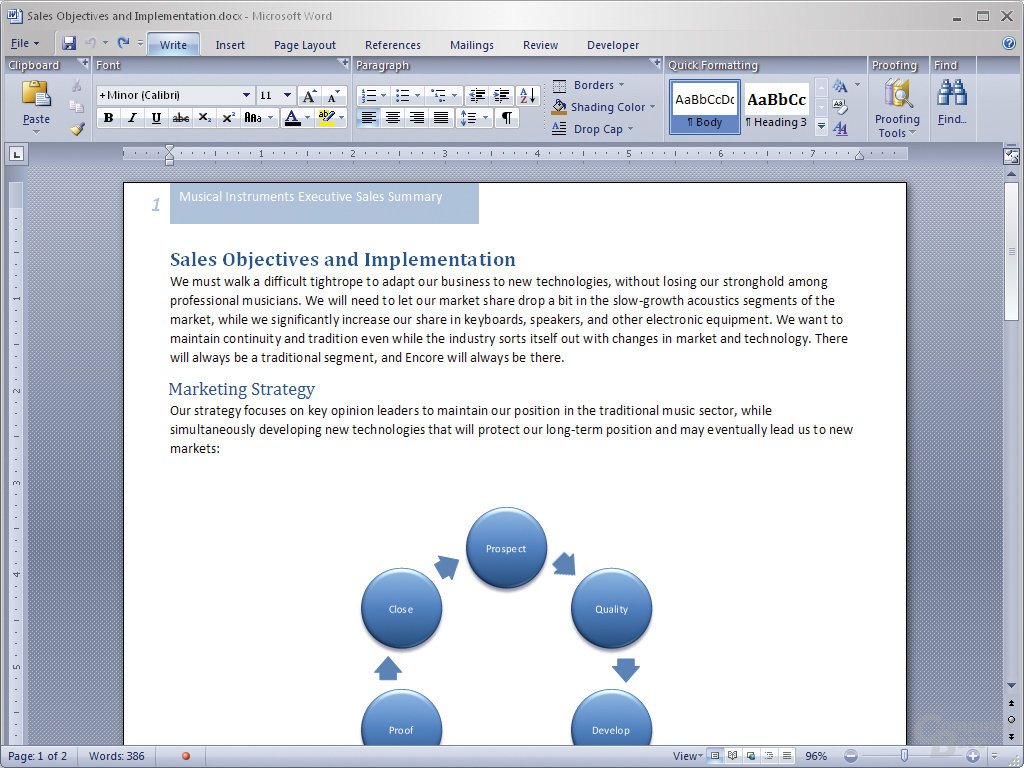
\includegraphics[keepaspectratio,width=\textwidth,height=\textheight]{office12.jpg}}
            };
        \end{tikzpicture}
	\nocite{office12,glitch,wikibsod}
     \end{frame}
}



\note{
	\begin{itemize}
		\item Imagine you're working on an important document and suddenly\dots
		\item Nothing is working anymore, your document probably lost.
		\item You don't perceive this as opportunity to learn more about Computers, how they work and why they fail
		\item It's not an invitation to get more familiar with them. (Even though it absolutely is.)
		\item It's the task that's important, the computer is just a way to solve a task, it should not be the cause of other problems that
			maybe you have no idea how to deal with
	\end{itemize}
}

\frame{
	Let's always remember this on our way to develop better software.

	Good software is that which does \textbf{not} annoy like that. And only good Software gets sold and used. This is why you should care.
}


\section[Follow the truth table]{Just follow the truth table!}

% what allows us to design CPUs is that we have a good theory of what the world is like. This allows us to construct things in our mind before testing whether those abstractions worked.
% This is the basis of all modern technology.

\frame{
	\begin{center}
		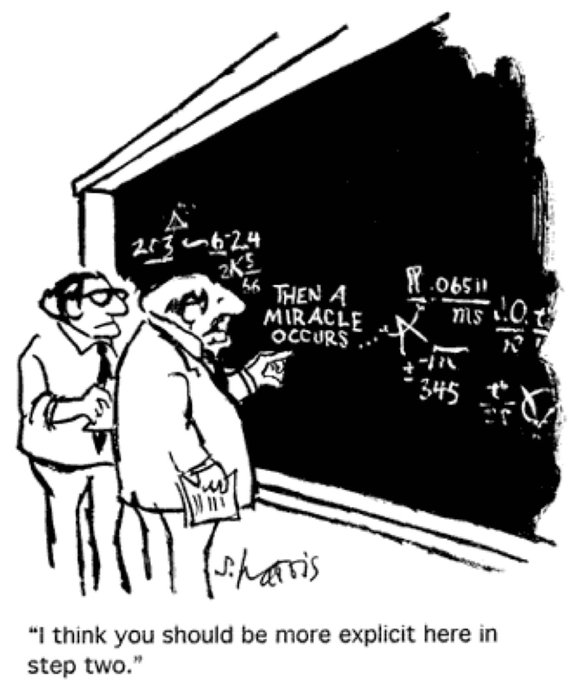
\includegraphics[height=0.76\textheight]{miracle.jpg}
	\end{center}
	\cite{thenamiracleoccurs}
}

\note{
	\begin{itemize}
		\item Before we can develop really good software, we need to demystify the computer.
		\item For some people computers are entirely like magic. You put something in -- then, magic happens -- 
			and you get something out
		\item Like there's a magic elf inside that solves these problems for you. Even for programmers.
		\item For some, like me, they're not \textit{entirely} magic anymore. I'm far from knowing
			all the details, but I think I got the gist of it right, and so I want to explain to you
			what a computer is, in philosophical terms, without the assumption of magic.
	\end{itemize}
}


\frame{
	\begin{itemize}
		\item I assume we have relays and switches.
		\item A switch interrupts a flowing current when it's in it's OFF position
		\item A relay has two inputs, a general-power input and a control input.
		\item It's function is to output power, once the control switch is on and not
			output power when it's off.
	\end{itemize}
}

\begin{frame}
	\begin{center}
		%\movie[width=10.35cm,height=5.811cm,poster,loop]{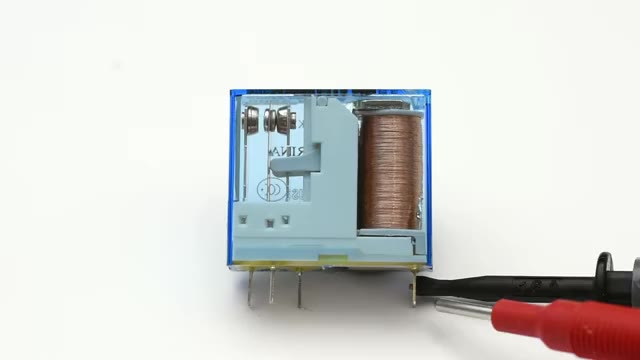
\includegraphics[width=10.35cm,height=5.811cm]{firstframerelais.jpg}}{relais.mp4}

		\href{run:relais.mp4?autostart&loop}{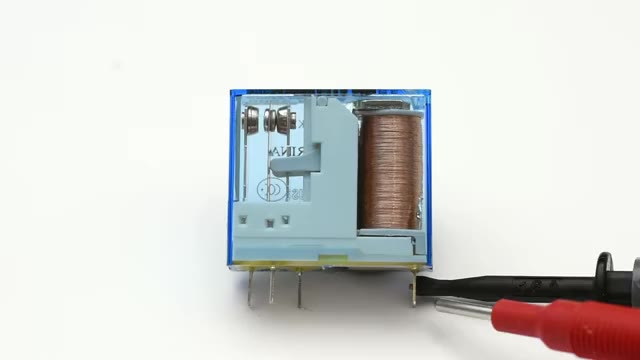
\includegraphics[height=0.7\textheight]{firstframerelais.jpg}}
	\end{center}
	\citetitle{wikirelais}
\end{frame}


\frame{
	\begin{center}
		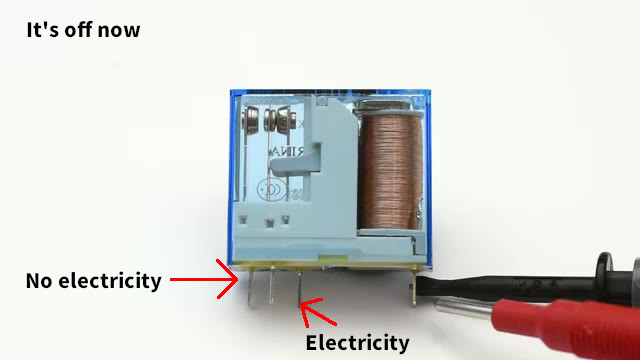
\includegraphics[width=0.7\textwidth]{not_relais.jpg}
	\end{center}
}

\frame{
	\begin{center}
		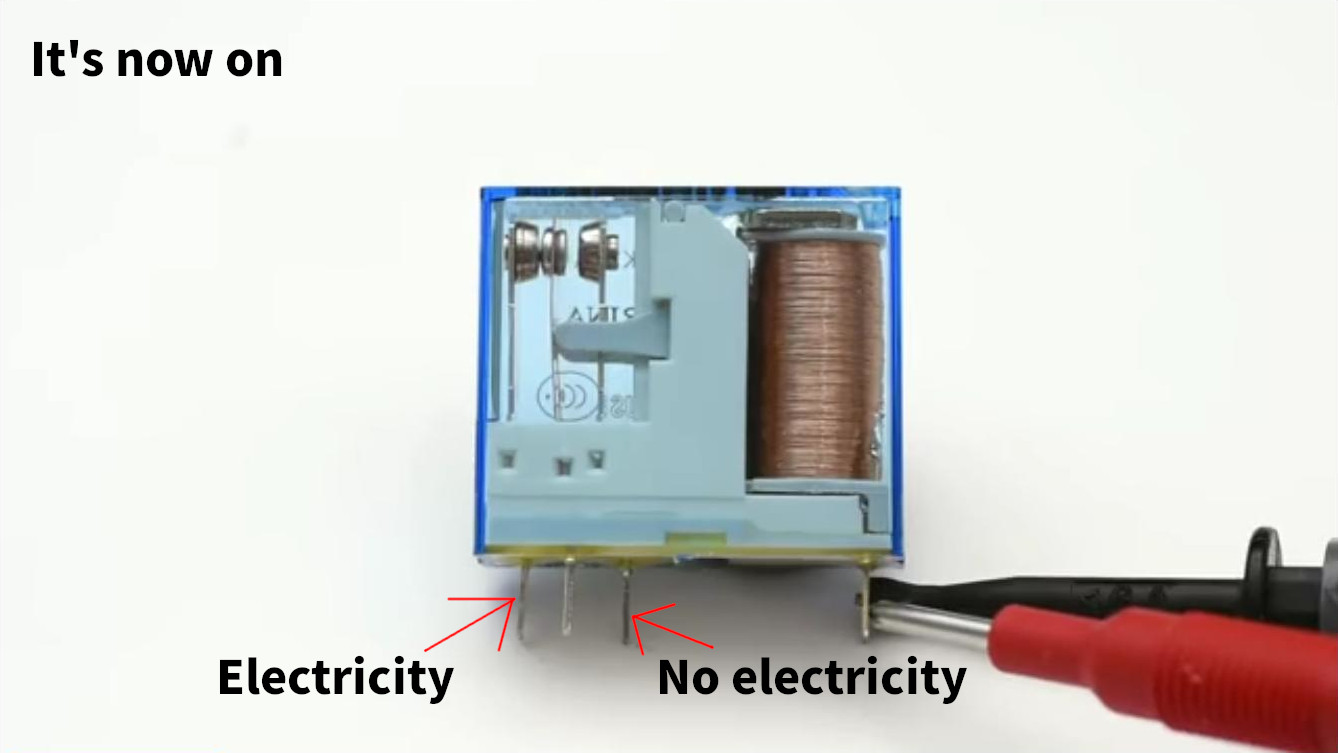
\includegraphics[width=0.7\textwidth]{relais_on.jpg}
	\end{center}
}

\frame{
	\begin{itemize}
		\item A function has an input-vector and an output-vector.
		\item $z = f\left(\begin{bmatrix}
				x\\
				y
		\end{bmatrix}\right) = \begin{bmatrix}
			x^2 \\
			x + y\\
			y^2
		\end{bmatrix}$ for example
	\item Or \texttt{AND}: $z = f\left(\begin{bmatrix}
			x\\
			y
	\end{bmatrix}\right) = \begin{bmatrix}
		x \wedge y
	\end{bmatrix}$
	\end{itemize}
}

\note{
	\begin{itemize}
		\item For this, let's very quickly turn to formal logic and math. I assume you have a basic idea of what that is.
		\item Let's imagine, our input $x$ and $y$ can only be one or zero, nothing else and keep the coventions for operations
			(this called a \textit{ring of integers of modulo n})
		\item We want to define one of the most basic parts of a CPU, an ALU (algorithmic-logical unit).
		\item There are many more parts to a CPU, like control flow units, but we are going to ignore those.
		\item Let's define an \texttt{AND}.
	\end{itemize}
}

\frame{
	Let's look at the truth-table of \texttt{AND}.

	\begin{table}[]
		\begin{tabular}{l|l|l}
			$a$ & $b$ & $a \mathrm{\ AND\ } b$ \\ \hline
			0 & 0 & 0       \\
			0 & 1 & 0       \\
			1 & 0 & 0       \\
			1 & 1 & 1
		\end{tabular}
	\end{table}
}


\note{
	\begin{itemize}
		\item See it? It's only true when both $a$ and $b$ are true.
		\item Let's construct this.
	\end{itemize}
}

\frame{
	{\Huge $a$ \texttt{AND} $b$:}
	\begin{center}
		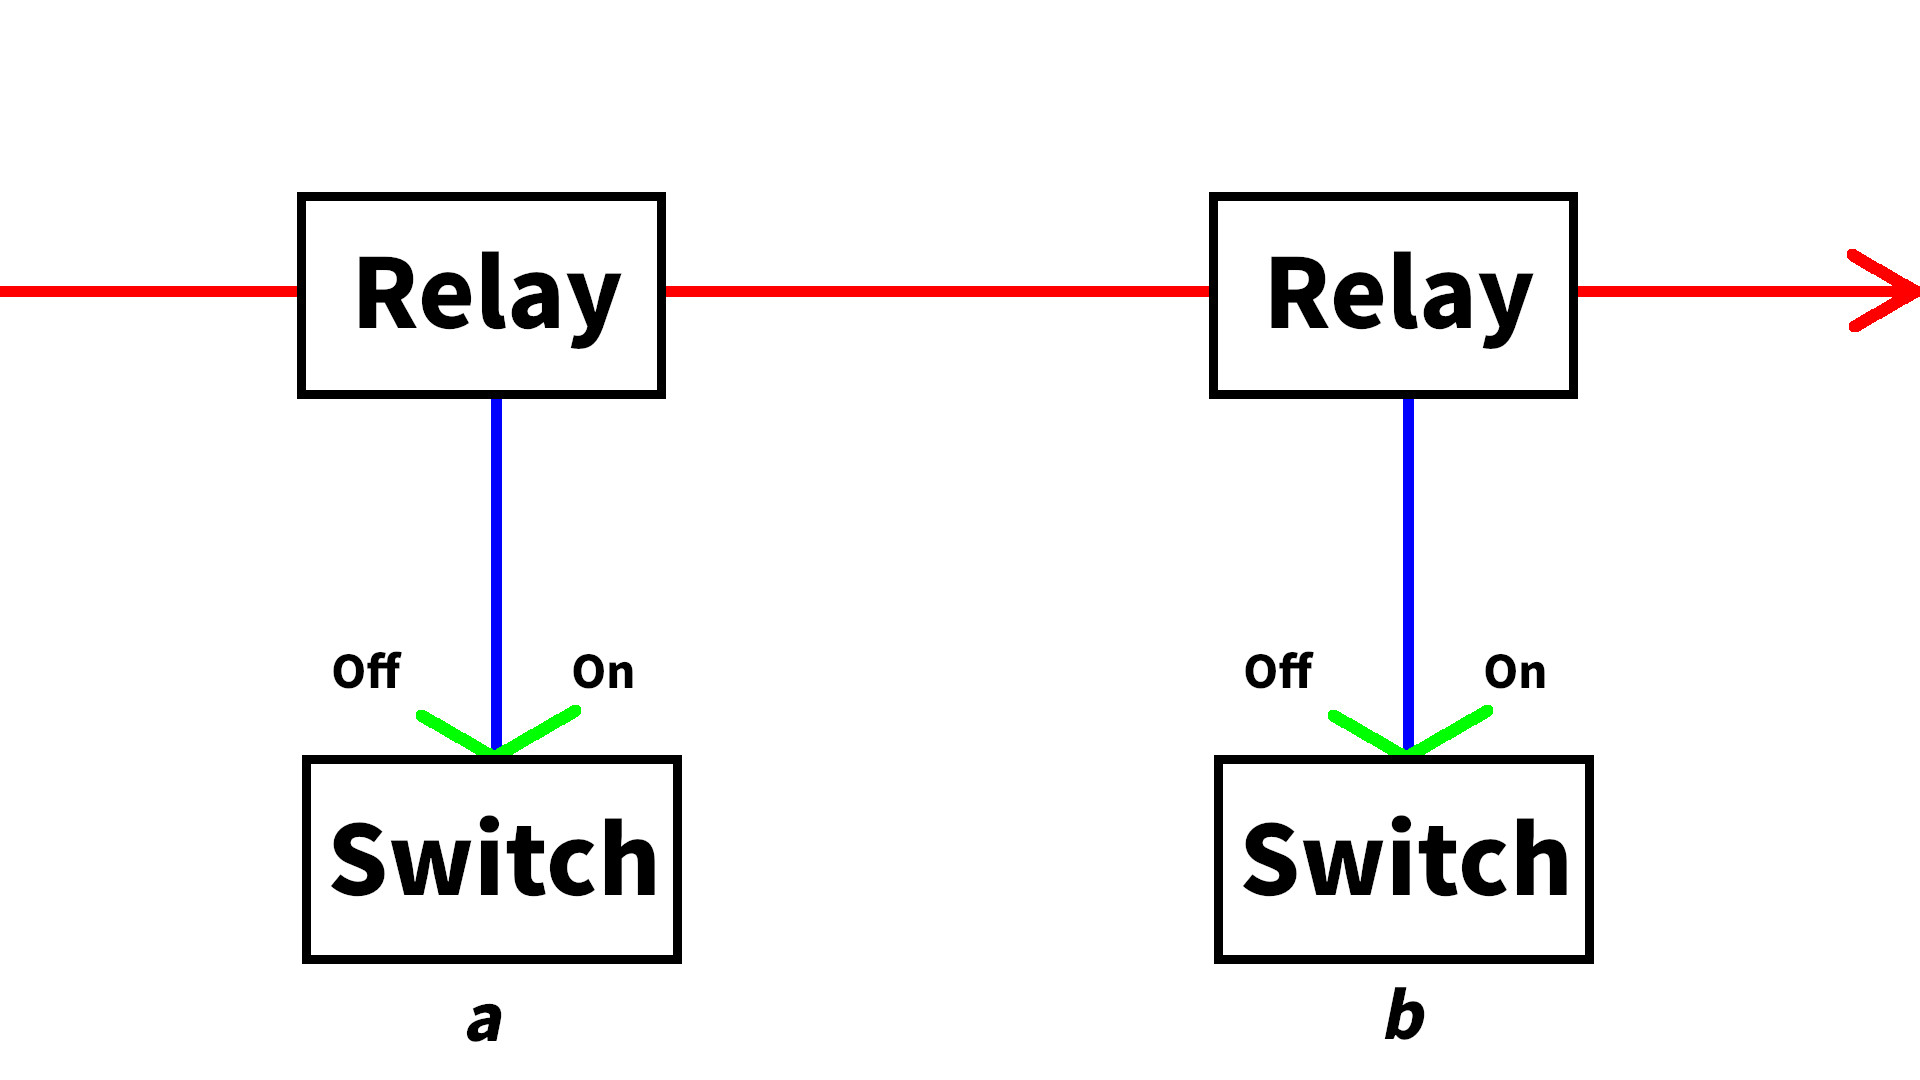
\includegraphics[width=0.8\textwidth]{and.jpg}
	\end{center}
}


\note{
	\begin{itemize}
		\item See? This can only be ON once both the $a$-switch and the $b$-switch are on. Otherwise, nothing comes out of this circuit.
		\item Now, this is not only a circuit, but the starting moment of modern computing.
		\item The idea is to use the natural laws of the universe (like the laws of electricity or flowing water) in such a way that they can 
			represent a truth table
		\item All modern computing is based on the creation of analogies of internal mental structures in the outside-world
		\item (I personally believe that this is because logic itself is an analogy of the world, so that we have the ability to manipulate
			things in our mind, and this ability is what differentiates humans from all other animals. Computers allow us to outsource
			the simplest form of thinking to a machine.)
		\item Only in the moment of inputting something and the moment of reading the outputs, the computer is really `calculating'. Inbetween,
			it's just doing physics.
	\end{itemize}
}



\frame{
	\begin{center}
		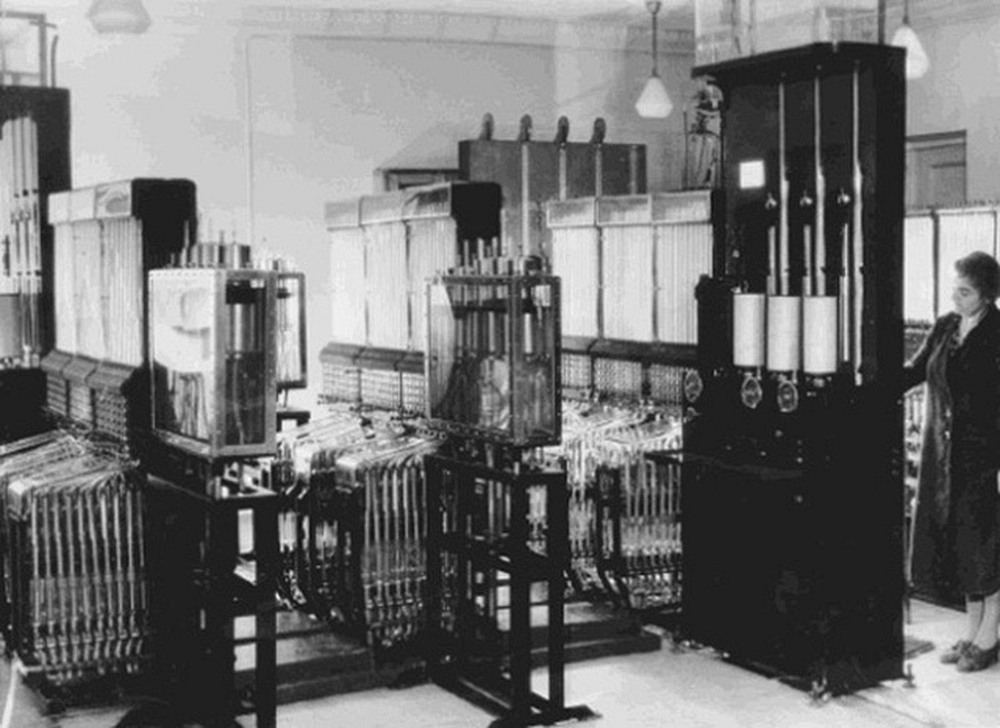
\includegraphics[width=0.6\textwidth]{integrator.jpg}
	\end{center}

	\cite{integratorbild}
}


\note{
	\begin{itemize}
		\item This analogy-idea of a computer can be transferred to quasi infinite many different ways.
		\item You can build computers with relays or with transistors. For the logic, it doesn't matter.
		\item You can even build computers that run on water, because you could choose water instead of electricity.
		\item This has been done btw.
		\item You even could build this from vacuum chambers and vacuum valves. With that idea, either there is a 
			good vacuum (1) or there's not (0). You can literally, in principle, compute anything computable
			with \textit{nothing}. You could run Linux on something that is the most \textit{nothing at all}
			we can achieve physically, if time and money were really no concern.
	\end{itemize}
}

\frame{
	Now let's define \texttt{OR} via it's truth table.

	\begin{table}[]
		\begin{tabular}{l|l|l}
			$a$ & $b$ & $a \mathrm{\ OR\ } b$ \\ \hline
			0 & 0 & 0       \\
			0 & 1 & 1       \\
			1 & 0 & 1       \\
			1 & 1 & 1
		\end{tabular}
	\end{table}
}

\frame{
	{\Huge $a$ \texttt{OR} $b$:}
	\begin{center}
		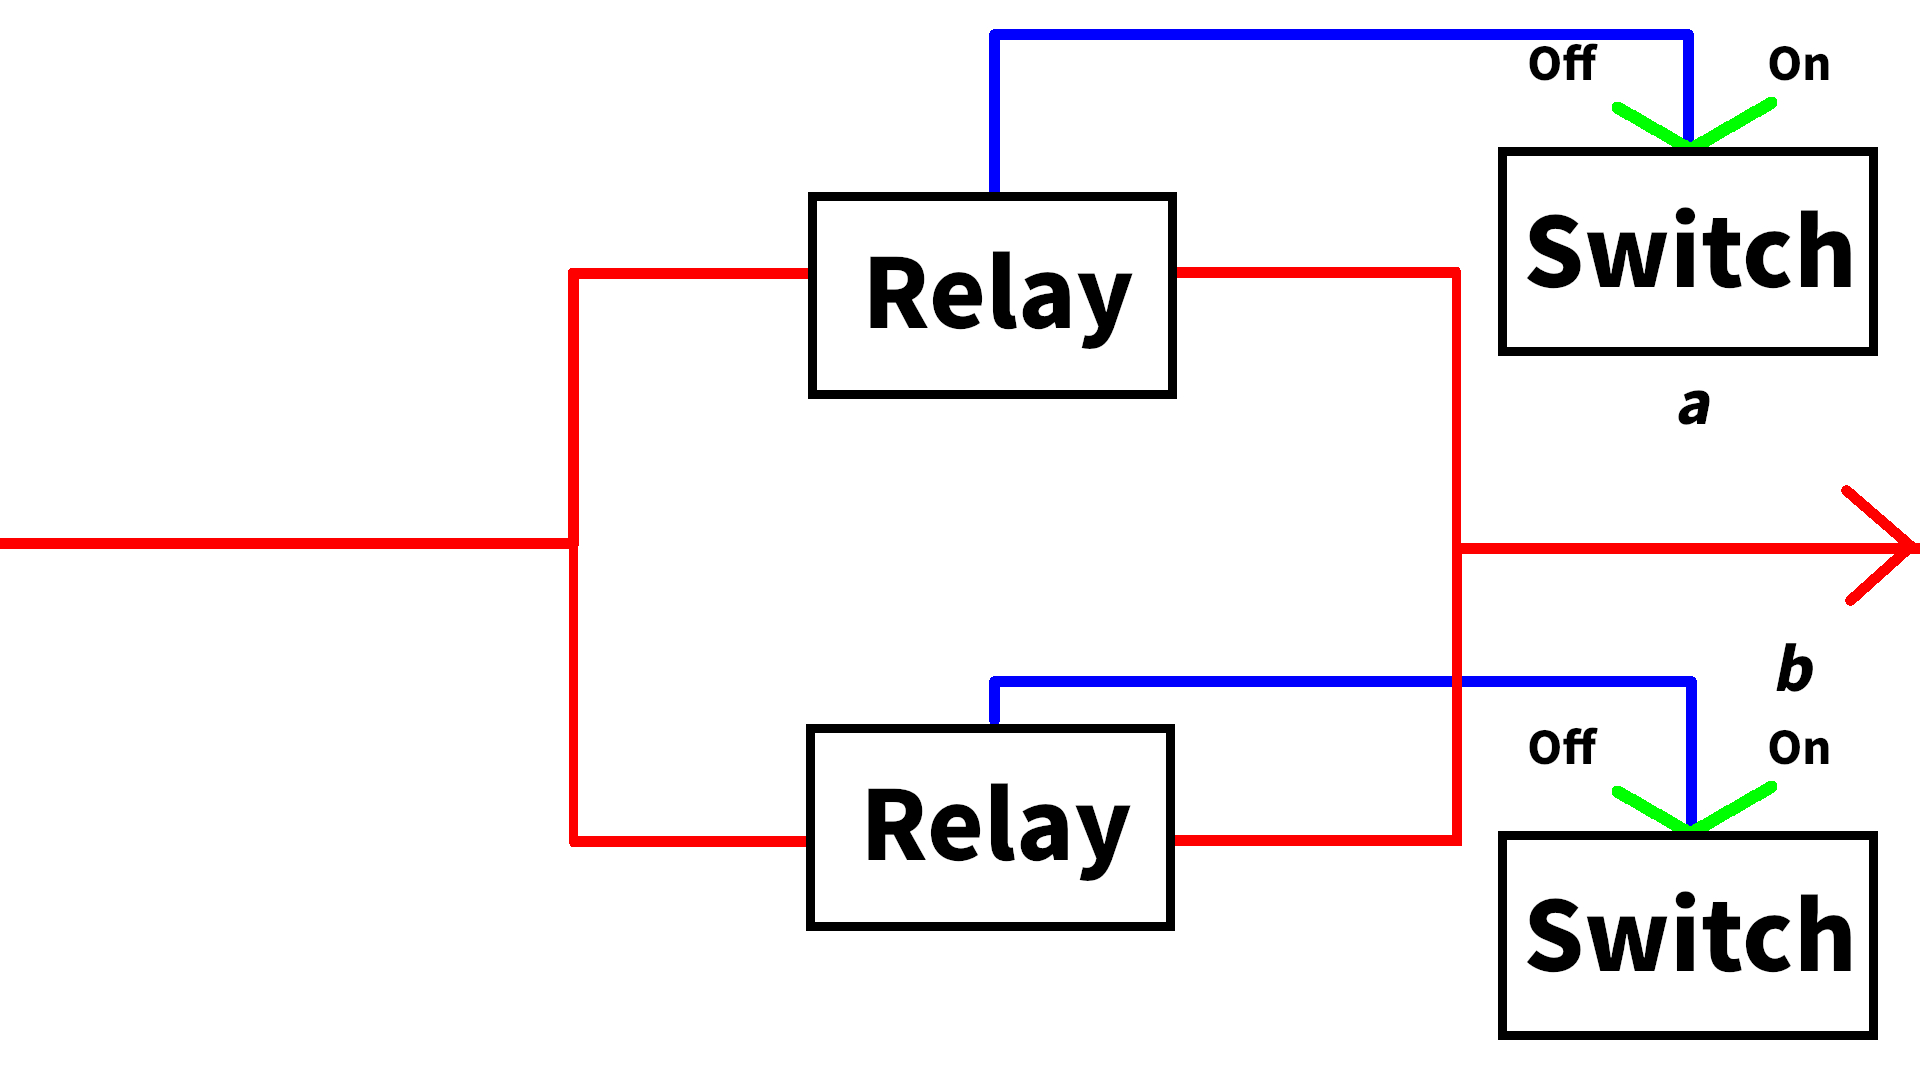
\includegraphics[width=0.8\textwidth]{or.jpg}
	\end{center}
}

\note{
	\begin{itemize}
		\item This is a logical OR. It is true when at least one input is true.
		\item At the end, there must be electricity (or water, or vacuum) if one or both switches are on.
	\end{itemize}
}

\frame{
	\begin{itemize}
		\item One last basic definition, but this one is very simple. Let's look at the truth table from \texttt{NOT}.
	\end{itemize}

	\begin{table}[]
		\begin{tabular}{l|l}
			$a$ & $\mathrm{NOT\ } a$ \\ \hline
			0 & 1      \\
			1 & 0
		\end{tabular}
	\end{table}

	\begin{itemize}
		\item This can easily be achieved by connecting the cable to the rightmost pin, so that there is no current flowing
			when the switch is on.
	\end{itemize}
}

\frame{
	{\Huge $\texttt{NOT\ } a$:}
	\begin{center}
		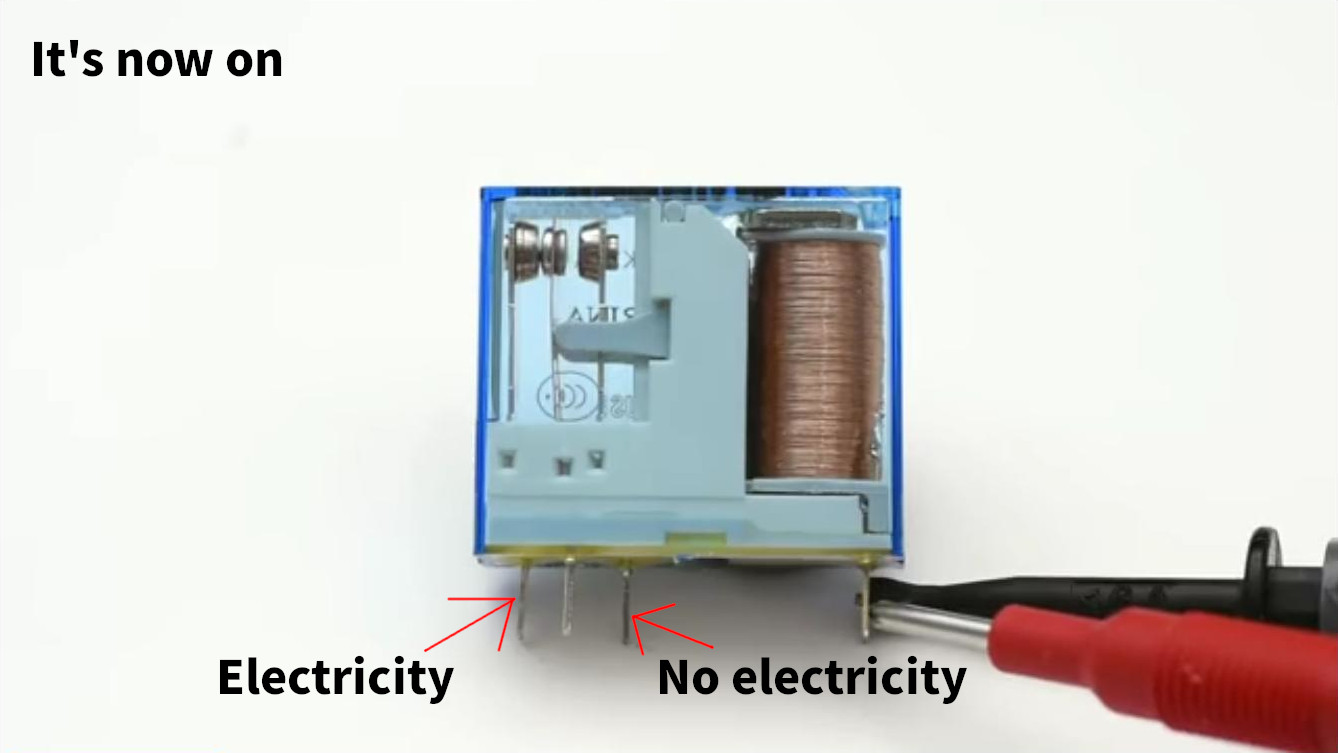
\includegraphics[width=0.7\textwidth]{relais_on.jpg}
	\end{center}
}

\note{
	\begin{itemize}
		\item See the three pins on the left? The middle one connects to the mains, and the left one is normally closed, and the right one is normally open.
		\item You can use the right one that is normally open as \texttt{NOT}. It only closes once the switch is in the on-position.
	\end{itemize}
}

\frame{
	\begin{itemize}
		\item Let's define \texttt{XOR}.
	\end{itemize}
}
\note{
	\begin{itemize}
		\item I hope you now see the connection between truth tables and the hardware and could construct something like this.
		\item Let us now go on even further a bit, but with equations only.
		\item Let's define \texttt{XOR}.
	\end{itemize}
}

\frame{
	\begin{table}[]
		\begin{tabular}{l|l|l}
			$a$ & $b$ & $a \mathrm{\ XOR\ } b$ \\ \hline
			0   & 0   & 0                  \\
			0   & 1   & 1                  \\
			1   & 0   & 1                  \\
			1   & 1   & 0
		\end{tabular}
	\end{table}

	\begin{itemize}
		\item You can see: \textit{it's only on when either (a is on and b off) or (a is off and b is on)}.
		\item $\left(a \mathrm{\ AND\ NOT\ } b\right) or \left(\mathrm{NOT\ } a \mathrm{\ AND\ } b\right)$
		\item We have all of these. So we do not need new hardware part designs, but only to merge already existing
			modules (\texttt{AND}, \texttt{NOT} and \texttt{OR}).
	\end{itemize}
}


\note{
	\begin{itemize}
		\item Imagine putting a lamp at the end of this.
		\item If we leave `is on', it is directly the logical notation equivalent to XOR. And this is all we need.
		\item From this, you can construct \texttt{XOR}. You now saw how each of them is realized. You've seen
			\texttt{AND}, \texttt{OR} and \texttt{NOT}.
	\end{itemize}
}

\frame{
	\begin{itemize}
		\item You can also now construct \texttt{NAND}, the negated \texttt{AND}:
	\end{itemize}
	\begin{table}[]
		\begin{tabular}{l|l|l}
			$a$ & $b$ & $a \mathrm{\ NAND\ } b$ \\ \hline
			0   & 0   & 1                 \\
			0   & 1   & 1                 \\
			1   & 0   & 1                 \\
			1   & 1   & 0
		\end{tabular}
	\end{table}
}

\frame{
	\begin{itemize}
		\item Or \texttt{NOR}, the negated \texttt{OR}:
	\end{itemize}
	\begin{table}[]
		\begin{tabular}{l|l|l}
			$a$ & $b$ & $a \mathrm{\ NOR\ } b$ \\ \hline
			0   & 0   & 1                 \\
			0   & 1   & 0                 \\
			1   & 0   & 0                 \\
			1   & 1   & 0
		\end{tabular}
	\end{table}
}


\frame{
	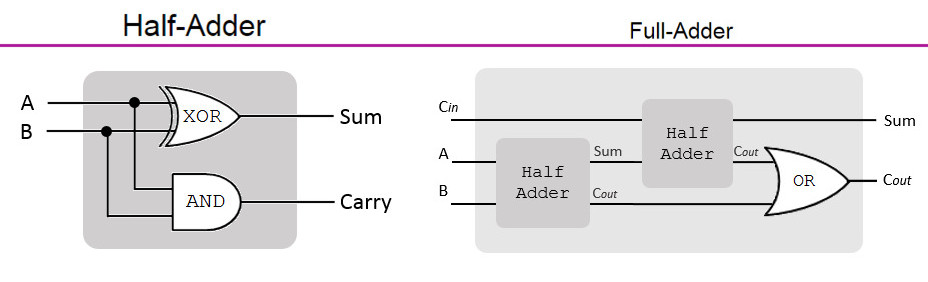
\includegraphics[width=\textwidth]{halfadderfulladder.jpg}
	\cite{halfadderfulladder}
}
\note{
	\begin{itemize}
		\item From \texttt{AND}s, \texttt{OR}s, \texttt{NOT}s and \texttt{XOR}s, you can build adders, subtractors, 
			multipliers and so on. Each one cares less about the direct implementation of the lower layers. It gets
			more abstract.
		\item The final layer should be the most abstract: the user-level of the program. You have good software when 
			the user does not need to worry about \textit{any} of the underlying details.
		\item And you can get more and more abstract (that is, removed from concrete hardware).
			Once you have a module you know acts like an Adder,
			just label it Adder and don't care about the exact underlying structure. Do this in all of your programs,
			so that the end-user does not need to care about implementation details in any way.
	\end{itemize}
}


\frame{
	\begin{center}
		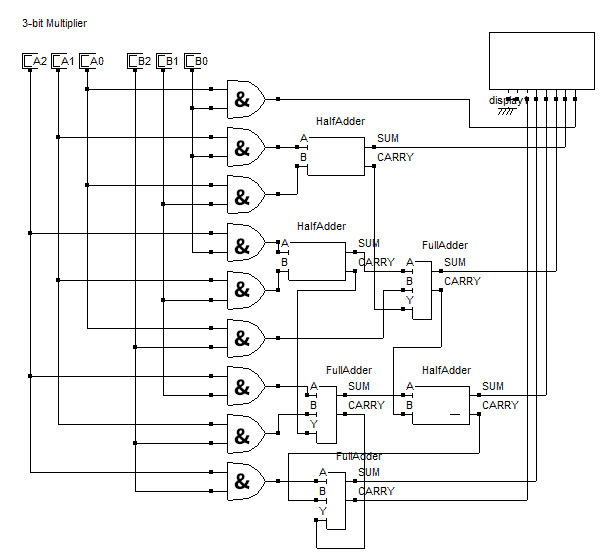
\includegraphics[width=0.5\textwidth]{mult.jpg}

		\cite{multiplier}
	\end{center}
}

\frame{
	\begin{itemize}
		\item For a general outline, we just need the \texttt{JMP}-instruction now.
		\item \texttt{JMP} is able to `jump' from one part of the code to another, similiar to \texttt{goto} in the basic idea
		\item Most CPUs define multiple jump-functions like \texttt{JE} (jump if equal), \texttt{JNE} (jump if not equal),
			\texttt{JG} (jump if greater), \dots
		\item With jump-instructions, you can do branches, very similiar to this Pseudo-Code:
	\end{itemize}
}

\begin{frame}[fragile]
\begin{lstlisting}[language=C]
if(a == 5) { // jump if a == 5
	goto A_EQUAL_FIVE;
} else { // jump if a != 5
	goto A_NOT_EQUAL_FIVE;
}
return;
A_EQUAL_FIVE:
printf("a==5");
return;
A_NOT_EQUAL_FIVE:
printf("a!=5");
return;
\end{lstlisting}
\end{frame}


\frame{
	\begin{itemize}
		\item When you have adders, you can build multipliers of them (as, with the integers at least, multiplication is just repeated addition).
		\item When you have multipliers and branch-statements like \texttt{JE}, you can use them to create a faculty function like that:
			$$
				n! = \begin{cases}
					1 & \mathrm{if}\ n == 1 \\
					(n-1)! & \mathrm{else}
				\end{cases}
			$$
	\end{itemize}
}

\frame{
	Assuming you also have a divison circuit, which we will also skip here, you can then build:

	$$\sin(x) = \sum_{n=0}^\infty (-1)^n\frac{x^{2n}}{(2n)!} = \frac{x^0}{0!}-\frac{x^2}{2!}+\frac{x^4}{4!}\mp\dotsb$$

	And with that work on even more and more complex structures, not caring about the detail-implementation anymore.
}
\note{
	\begin{itemize}
		\item This is what libraries do for you.
		\item When you do $\sin(x)$ in C, it gets breaken down to the taylor series shown
		\item This then gets broken down to a lot of \texttt{AND}s, \texttt{XOR}s and \texttt{NOT}s.
		\item Programs as I think most programmers understand them are usually only `glueing together' libraries,
			things that abstract away from the hardware that you don't have to think about the logical implementation.
		\item When it's there, the $\sin$ can be used to calculate all kinds of things. Every 3D-game you ever played used these
			as libraries for the graphics for example. And the developer did not need to re-invent the wheel.
	\end{itemize}
}


%\frame{% TODO
%So the reason you can do this
%	% https://youtu.be/erc1Qrjl1oY
%	is the development of math of the last 2000 years,
%	and of logic for the last 2500 years
%	and finally because of this guy:
%	aristotle,
%	who first had the idea of formalizing logic.
%}


\frame{
	\begin{center}
		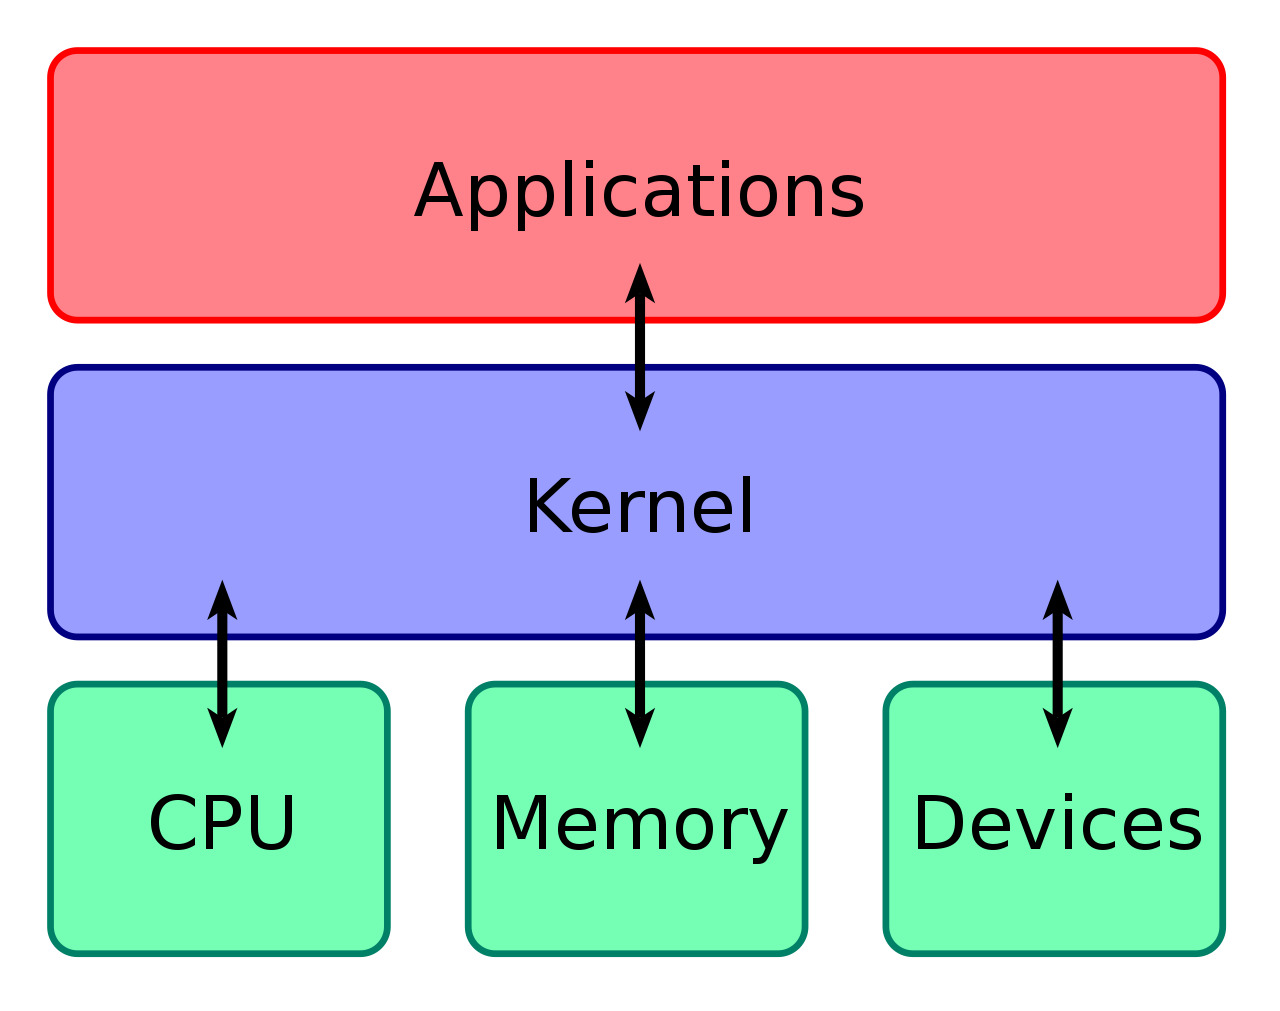
\includegraphics[width=0.8\textwidth,height=0.8\textheight,keepaspectratio]{kernel.jpg}
	\end{center}
	\cite{wikikernel}
}
\note{
	\begin{itemize}
		\item The quest for more and more abstract ways of programming leads us to operating systems.
		\item An OS is a piece of software that abstracts away the concrete hardware.
		\item The \textit{kernel} is what communicates with the hardware, and your software communicates
			with the kernel.
		\item The kernel allows you to execute certain commands, abstracted away from the real hardware,
			so you don't need to care about a specific implementation of \texttt{AND}s and \texttt{XOR}s, but only
			about doing basic level mathematics for example.
	\end{itemize}
}

\frame{
	\begin{center}
		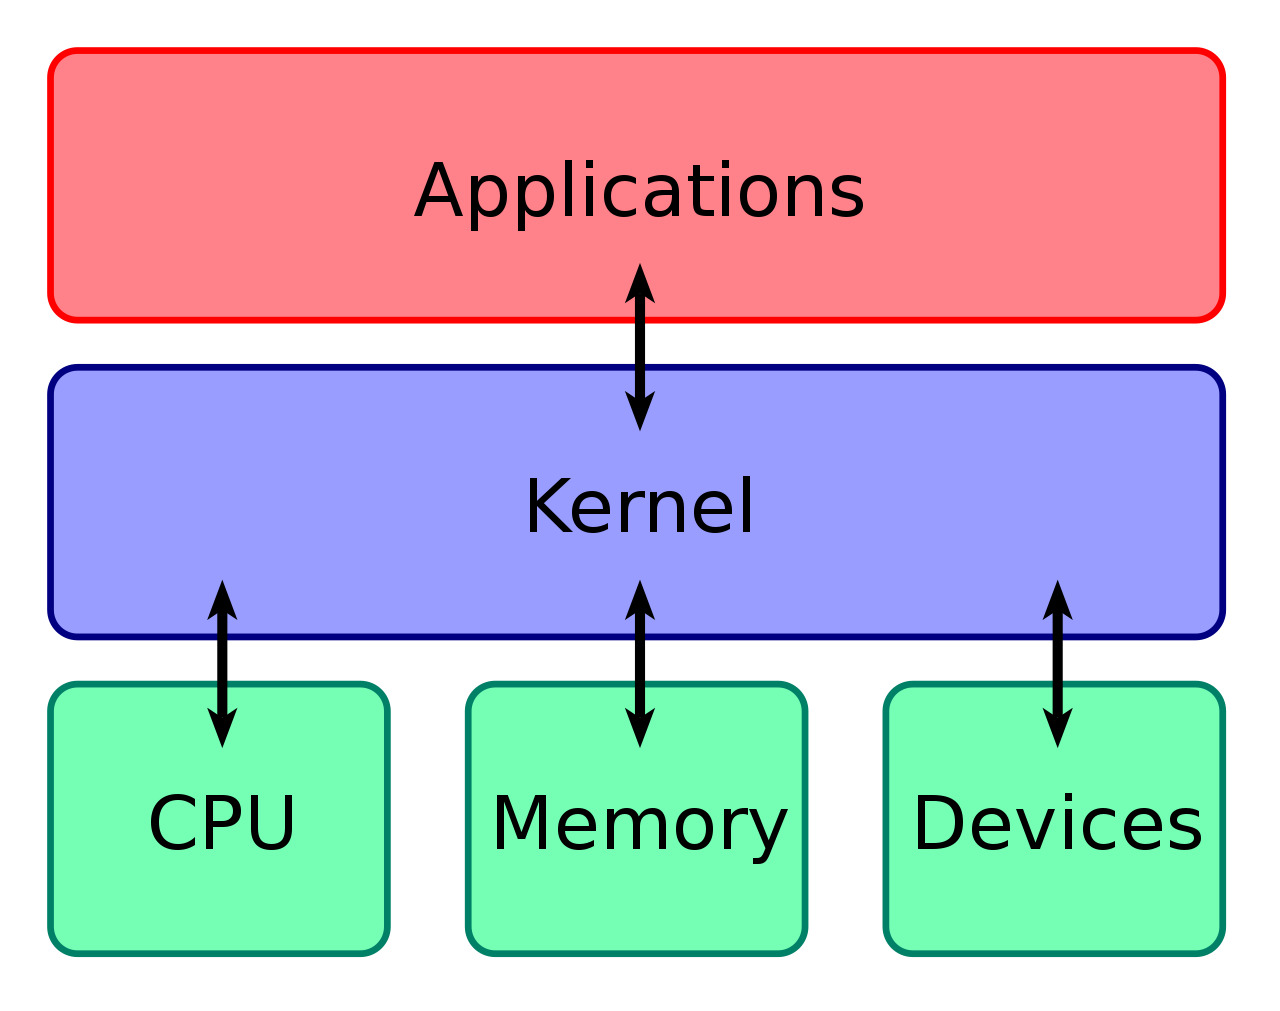
\includegraphics[width=0.8\textwidth,height=0.8\textheight,keepaspectratio]{kernel.jpg}
	\end{center}
	\cite{wikikernel}
}
\note{
	\begin{itemize}
		\item Having a kernel has the advantage that you don't need to care about communication with the hardware, only
			with the kernel. The kernel communicates with the specific hardware for you.
		\item The OS also allows you to communicate with other hardware, like printers, over a generalized
			interface. The OS needs a driver (a piece of software that tells the kernel how to use certain pieces
			of hardware), and then you can use the OS's features with that hardware, without caring about
			the intricacies of the printer.
	\end{itemize}
}


\frame{
	\begin{itemize}
		\item This is also what higher-level-languages do.
		\item The idea of a high level programming language is that, for programming them, you don't need to care about implementation details.
		\item They abstract things away from you. And I guess it's easier to find a python developer than a assembly-expert because of exactly that.
		\item Coding in assembly is much harder because you need the ability for higher mental workload.
		\item Not only the problem you really care to solve, but also additional problems (implementation details)
	\end{itemize}
}

\note{
	\begin{itemize}
		\item Please always remember that all of this would not have been possible without philosophers like
			Aristotle, who first had the idea of formalizing logic, or George Bool, who first researched
			`boolean arithmetic', or Descartes, who first researched function theory.
		\item Most of those discoveries were, at their time, regarded as `useless'
		\item See `\citetitle{hardy1967mathematician}' by G.~H.~Hardy (1940), in which he claims that number theory,
			is one of the most beautiful mathematical areas, despite it not \frqq\textit{being able to be used for anything}\flqq
		\item He was right and wrong at the same time. It is the most beautiful mathematical area, but today also
			one of the most useful ones. Without developments in number theory, the internet would not have been
			possible as it is today (no cryptography would be possible without advancements in math made some houndreds or even
			thousands of years ago that, at their time, seemed useless to most people).
		\item So remember, sometimes `the most useless' things may turn out to be the most useful things to later generations.
	\end{itemize}
}


\fullpageimage{white}{vonneumann.jpg}{wikivonneumann}

\note{
	\begin{itemize}
		\item What I've skipped:
		\item My description of what a computer is is far from complete here. For it to run as you are now used to, you need memory, for example,
			and you need way more transistors than I could possibly draw. Also, you need a control unit for your CPU. And so on.
		\item But this should give you just the right gist of thinking about the central part of your computer that is usually more mystified than
			clear to most people.
		\item If you want to learn more about this, search for \textit{Von-Neumann-Architecture}. This here was just intended to demystify the
			very basics.
	\end{itemize}
}

\frame{
	\begin{itemize}
		\item What does this practically mean?
		\item You must try to \texttt{catch} any errors you can imagine. Assume everything can -- and will -- fail all
			the time in every conceivable way. And also in all ways that you did not consider.
		\item Did you, for example, know that \texttt{fork()} can fail and that, if not properly treated, has 
			disastrious consequences?\footfullcite{forkcanfail}
		\item Also assume everything that can be entered by a user is garbage. They'll add numbers in fields designated for
			letters, they enter $0$ in a field through which something is divided and they'll try to \texttt{chmod +x}
			and run any \texttt{jpeg}-file they own and run them with sudo.
	\end{itemize}
}

\frame{
	\begin{itemize}
		\item Also really make sure you trust your subcomponents. Proving every algorithm is not do-able in practice, but write
			as many unit tests as you can. And test the interaction between modules, too. Best auto-test all of the programs
			features.
		\item Write each positive and negative tests, so that you can test your error routines.
			If you find bugs, write a test that matches them first, and then fix them. Then you can test for the presence and absense
			of that bug.
		\item Monkey-Test your script. For webpages, I recommend \textit{gremlin.js}. You can run a simple piece of code and it will
			click randomly and enter anything into any field and press any key randomly, with as many workers in parallel as you wish.
			\begin{itemize}
				\item For X11 applications, you may look into \texttt{xdotool} (or \texttt{ydotool} for wayland).
			\end{itemize}
	\end{itemize}
}

\frame{
	\begin{itemize}
		\item You cannot trust anything from the outside. Don't assume a User will only use \texttt{ASCII} in his folder names, but
			assume strange \texttt{UTF-8} symbols from a russian encoded website from a buggy browser that modifies random bits. It must either
			work, if you really find no way of making it work, display an exact error message on what's wrong and what needs to be done
			about this. (When writing GUI-Applications, make it easily copyable so that it can be googled).
		\item Like in real life, you cannot stop things from going wrong. But you can stop them from going horribly wrong. You can catch most
			of the `wrongness' if you clean up after yourself properly and don't rely on other people to do your work
	\end{itemize}
}

% Suspect that everything will go wrong. Literally EVERYTHING. Check return-values. Use exceptions. Compile a debug-version of your software where every warning leads to hard crashes. Ideally, there should not be any warning left when you use your program. Then compile a version of it where warnings do not crash the program. Distribute that. But test with FATAL WARNINGS.

\section[Phenomenology]{What is \frqq Phenomenology\flqq?}

\fullpageimage{black}{heidegger-crop.jpg}{heideggerbild}
\note{
	\begin{itemize}
		\item Heidegger was the first philosopher to criticize the european philosophy at it's fundamental level.
		\item He said, from Plato on, philosophers have lost track of `real life', focussing on abstractions instead.
		\item Using abstractions is easier of course, but an abstraction can never replace real life.
		\item He called it `Seinsvergessenheit', the forgetting of being itself.
	\end{itemize}
}

\fullpageimage{black}{heidegger-crop.jpg}{heideggerbild}
\note{
	\begin{itemize}
		\item You can think about riding a bike, or ride a bike. They're not the same at all.
		\item This is called ontic-ontological difference. Ontic refers to `what we really do`, ontological is `thinking about what we really do'.
		\item The task of philosophy is, according to Heidegger, to get the the focus to the real life instead of just thoughts about real life.
	\end{itemize}
}

\fullpageimage{black}{heidegger-crop.jpg}{heideggerbild}
\note{
	\begin{itemize}
		\item This is what we have to keep in mind for good software, too. 
		\item Move away from what you think users want and are to what users really want and are.
		\item This is not easy, since most of the time they don't know it themselves.
		\item But it can be achieved by observation of yourself, since you are also `just' a user of your own software.
		\item And it can be achieved by outside user's with different mindsets and goals via communication.
		\item Schmitz, a successor of Heidegger, has really started this focus on real life, in my opinion.
	\end{itemize}
}

\fullpageimage{black}{schmitz.jpg}{schmitzbildwiki}
\note{
	\begin{itemize}
		\item This is Hermann Schmitz.
		\item He's a comtemporary german philosopher who invented `the new Phenomenology'
		\item Sadly, he passed away on the 5. of may 2021 at the age of 92.
		\item His ideas in short terms were:
		\begin{itemize}
			\item We are not merely our rationality, nor are we merely our body. 
			\item Our rationality is that which thinks most often in words inside our head.
			\item Our body is that which a doctor palpates when he examines us.
			\item What's missing is our \textit{subjective body}. If a loved one touched you exactly the same
				as a doctor may touch you, it may feel very different.
			\item The subjective body is our experience of our body \textit{and} our mind.
		\end{itemize}
	\end{itemize}
}

\fullpageimage{black}{schmitz.jpg}{schmitzbildwiki}
\note{
	\begin{itemize}
		\item Do you know phantom pain? 
		\item If someone loses an arm due to an accident, it would be logical to think that he does not feel it anymore.
		\item But this is not the case. People who lost limbs often report still feeling the pain in them.
		\item This is because though they lost a part of their physical body, it is still part of their \textit{subjective body}.
		\item In this \textit{subjective body} we experience all our emotions and atmospheres.
		\item All of live is basically just a row of following situations in certain spaces, submerged in atmospheres.
		\item This is important to notice. You cannot not be in a situation. You cannot not be in an atmosphere.
			They sorround you all the time. 
	\end{itemize}
}


\fullpageimage{black}{schmitz.jpg}{schmitzbildwiki}
\note{
    \begin{itemize}
        \item Atmospheres and situations, not physical matter, primarily constitute reality as we experience it
        \item The new idea of Phenomenology is to treat experiences as real. The pain you may experience is as real as the chair your sitting 
            on
        \item They are in different categories, since you have access to that chair, but not my experiences, but they are nonetheless
            the realest reality I can get
        \item If you are in severe pain, the pain is much more real to you than a mathematical proof
        \item Good programs create a good atmosphere. Programs that create bad atmospheres (by, like, crashing, or acting unexpected)
            are bad programs.
    \end{itemize}
}



% TODO!!!! Im Video Sound einbinden. creepy.mp3!!!
\fullpageimage{black}{creepy.jpg}{creepyimage}
\note{
	\begin{itemize}
		\item !!! Add creepy music here !!!
		\item Imagine walking through this abandoned insane asylum in the night without a flashlight, hearing weird sounds
		\item Do you feel that constricting feeling in your chest-area? This is your \textit{subjective body}s reaction to 
			that creepy, weird area.
		\item The german Word `Angst' is etymologically derived from the same word as `Enge', which means `narrowness',
			because it's connected to this constricted feeling.
	\end{itemize}
}

\fullpageimage{white}{euphoria.jpg}{wikieuphoria}
\note{
	\begin{itemize}
		\item Or have you ever felt like this? Liberated, euphoric, happy to be alive?
		\item The feeling in your chest-area might be liberating and widening.
		\item According to Schmitz, these are the most general ways of subjective body states:
			between absolutely constricted, and absolutely open
		\item You need both in life, like the expansion of the Leib when breathing in in swelling of the fealing chest-area, that would be
			unbearable if it wouldn't be exhausted just right after, resulting in in wave of experiences of widening and narrowing Leib
		\item Usual situations are a complex mixture of states between those extremes in different what Schmitz calls 'Leibliche Region', like the lost arm with phantom pain, ``that are in the area, but not neccessarily in the borders of the body''.
		\item Whether you feel fear, or you are happy or liberated, it is always a feeling that affects the Leib
	\end{itemize}
}


\fullpageimage{white}{euphoria.jpg}{wikieuphoria}
\note{
	\begin{itemize}
		\item These are the most basic extremes of life. This is the best that 4 billion years of evolution
			could produce to tell us about our sourroundings.
		\item We should start to use it properly!
		\item That is, have our inner focus properly adjusted to experiences.
		\item If you use your software, and something annoys you, which you can fix, \textit{fix it}! (This is a generally good tip for life)
		\item But you have to really use the software. And see how other people use your software. They'll often don't see things that 
			seem `obvious' to you because your so involved with your code.
	\end{itemize}
}

\fullpageimage{white}{euphoria.jpg}{wikieuphoria}
\note{
	\begin{itemize}
		\item They also see things that are obvious to them, but not to you, since you are not thinking like them, because you are not them.
		\item Heidegger calls this ``Jemeinigkeit'', the \textit{Dasein}, i.\,e. \textit{you} as a human being, is always experienced from 
			the subjective perspective that is always \textit{mine} (from the person observing)
	\end{itemize}
}


\fullpageimage{white}{rtfm.jpg}{wikirtfm}
\note{
	\begin{itemize}
		\item In theory, users have an infallible memory system. And they read manuals before using the program. They know exactly what they want 
			and how to achieve it the most efficient way possible.
		\item But in reality they are never like that. 
		\item Do you read a 400 page manual before using a `simple' program? I do not. Nobody wants to read a manual to
			use a webbrowser. It's just a tool that needs to do it's job. And of course real humans always forget and barely ever know
			what they want exactly.
		\item It's not like when you play music on Youtube, you want to think about how the https-protocol is implemented. You only care about
			the music.
	\end{itemize}
}

\fullpageimage{white}{rtfm.jpg}{wikirtfm}
\note{
	\begin{itemize}
		\item Thinking is a very complex task and requires a lot of effort that the people using software would rather like to spend
			on the problem they try to solve \textit{with} the computer
		\item I believe we developed consciousness evolutionary to have the ability to focus on problems that we cannot solve by intuition alone.
		\item Remember when first learning to drive a bike or a car? You had to do everything very consciously, until it went `down in
			your nervous system' so that you do the things correctly without thinking about them. When consciousness fulfils it's
			duty of learning, we can disable it and drive on auto-mode mostly.
		\item The task of consciousnes is, as Zen buddhism puts it, to get rid of consciousness.
		\item This is what he have to achieve with our software, so that people will use it without having a learning curve. If your
			users always use the program wrongly, they think different about the problems than you, and your task is to bridge that
			gap by making it work the way people think.
	\end{itemize}
}

\fullpageimage{white}{rtfm.jpg}{wikirtfm}
\note{
	\begin{itemize}
		\item Real humans have a very limited ability for mental workload. They can only keep some very few things at the same time in their head, and usually
			the computer is one of those that they have to have in their head, but don't want it there, because they don't have the goal of
			using the navigation software, but of reaching the goal \textit{with the navigation software}.

		\item They want a result on the level of analysis they look at right now
		\item If you drive a car and it breaks down, you have to change your level of analysis. From \textit{this is an object that gets me from $A$ to $B$},
			you must suddenly switch to \textit{this object has an engine with like a billion parts and complex circuits and all that stuff, what do now?}.
		\item A good car is one where you don't have to switch the level of analysis. And this is also the trademark of great software.
	\end{itemize}
}


\fullpageimage{white}{hegel.jpg}{wikirtfm}
\nocite{hegeldeutschlandfunk}
\note{
	\begin{itemize}
		\item Hegel wrote an article about abstractness and concreteness (\cite{hegelabstrakt}). He said, usually people think the abstract thing is the hard one, like abstract mathematics, and the concrete is the easy one. He argues that often it's the opposite.
		\item For example, checking my average school marks vs. the ones' of another one is easy. But looking at whether the person is right in that job, that's hard.
		\item Abstract means, we exclude. It is etymologically derived from abstrahere in latin, which means to 'cut away'. Abstract means we can concentrate on only one or at least very few factors.
		\item Abstraction is great, because then we can see parts of the future and develop towards them, even though they are not here yet. This gives us the vision to do things. But it comes with the price that we all-to-often forget the reality, fall for Heideggers' `Seinsvergessenheit', and confuse our image of the world with the real world.
	\end{itemize}
}

\fullpageimage{white}{hegel.jpg}{wikirtfm}
\note{
	\begin{itemize}
		\item In software, we want exactly \so{this} abstraction.
		\item Good software cuts away everything from you that you don't care about while solving the problem
	\end{itemize}
}

\fullpageimage{white}{tunnelradio.jpg}{wikirtfm}
\note{
	\begin{itemize}
		\item Do you know the feeling of flow? When you do something and everything works as expected and helps you to fulfil your goal?
		\item Sometimes, when driving through tunnels, you see signs that the radio will not work. 
		\item You want to drive a car and listen to radio. Of course you know why it has problems. You kind of know how the radio network works.
		\item But This is an interruption nonetheless. Where the flow is interrupted.
		\item NEVER EVER BREAK THE FLOW
		\item Flow-breakers are needing to think about the implementation of something that you just want to use, like the navigation software,
			or they even outright stop working, like the radio.
	\end{itemize}
}


\fullpageimage{white}{tunnelradio.jpg}{wikirtfm}
\note{
	\begin{itemize}
		\item Every time something breaks the flow, fix it.
		\item We cannot expect all our users (and ourselves) to become full ``zen-monk-flowy''. So we have to take care about all the situations that break the 
			flow by fixing them.
		\item Think in user-perspective. The user does want to solve a problem, not first create a bunch of other problems for himself.
		\item While there are flow-breakers, fix them. Fix the most severe ones first (like not being able to start the software
			without a bluescreen).
		\item The second biggest flow-breaker has become the most important show-stopper now, which you also fix. The software is 'done'
			if neither you nor the end users (or a test group of normal users) find some other flow-breakers.
		\item (But in reality, it's never done.)
	\end{itemize}
}


\fullpageimage{white}{tunnelradio.jpg}{wikirtfm}
\note{
	\begin{itemize}
		\item Eat your own dogfood! Actually use your software. And look at how end-users will use it. They will think about it
			differently, because they don't have the knowledge about it you do.
	\end{itemize}
}

\fullpageimage{white}{speechrecognition.jpg}{speechrecognitionimage}
\note{
	\begin{itemize}
		\item Things like speech recognition does all of this. The user does not have to think about a machine as machine,
			but can only say what they want
		\item With the rise of language models like chatGPT, this development is much further driven than ever imagined in scifi-movies already.
		\item This abstracts away completely even from using the `normal' interface
		\item This is Google's trick. You don't need to care about implementation details at all.
		\item The web usability tester Steve Krug said about this: `Don't make me think!'
		\item This is the secret.
		\item Good software is the software that doesn't make you think
	\end{itemize}
}



%\section[\google]{Then now, why is \google\ so successful?}

\frame{
	\begin{itemize}
		\item Because \google s founder's the world phenomenological, probably without realizing it.
		\item They wanted to solve a real problem, finding information, on the real internet as quickly and with as little hassles as possible.
		\item It's pure phenomenological Software testing with the goal of solving a problem in as little steps as possible.
	\end{itemize}
}

\frame{
	\begin{itemize}
		\item They see a problem. You are outside, away, and need a timer for something. You always have smartphone with you, would be great if it
			had a timer. So they add one.
		\item Tired of typing with cold fingers, very slowly on a screen? Develop speech recognition.
		\item And now you can add those. You can teach the speech recognition to set a timer for you.
	\end{itemize}
}

\frame{
	\begin{itemize}
		\item Maybe you want to go out sometimes, go for a fully new place. It would be great to have a digital map and a navigation website.
		\item Yeah, use \google\ Maps. You can even use speech recognition for the map, and output your speech so that you don't have to read.
	\end{itemize}
}

\frame{
	\begin{itemize}
		\item When you drive somewhere, the goal is not the interaction with the navigational system, but it's reaching the actual goal. The navigation is just
			a thing that you need to reach a goal convienently and it should annoy you as little as possible.  
		\item What they do: they continue the road laid out in the CPU-Design-Part. They abstract the concrete details the most away from you as possible
			because most people don't care about those details. They just want a quick result.
	\end{itemize}
}



\section[Summary]{Summary}

% There are different modes of being. One is the flow, another one is distress. We dislike distress and like "the flow". In "the flow" we concentrate fully on what we do, and achieve exactly what we want to achieve. The flow is one of the most basic things that tell us that something is good, and distress, which destroys the flow, is one of the most basic things that tell us something is bad.

\frame{
	Good software has these 2 properties:
	\begin{itemize}
		\Huge 
		\item it is as abstract as possible,
		\item it \textbf{never} breaks the flow!
	\end{itemize}
}

\frame{
	Those are the steps from a phenomenological standpoint that you have to follow to create good software:
	\begin{itemize}
		\item Look what you yourself (and others with other mindsets) \textit{really} do and fix the program until it matches the
			way people who will use the software think
		\item Try seeing what `annoying' means by completing the userinyerface.com task to `register'. You will learn a lot by doing this.
	\end{itemize}
}


\printbibliography[title={Sources}]

\end{document}

% Hallo Norman, ich habe ein paar Anmerkungen wegen des Beta-Tests: Bei den Relais-Sachen fehlt irgendwie der Übergang zur Software. Du bist da auf der Ebene von Schaltungen und machst dann einen weiten Sprung zu Funktionen und Software. Da könntest du noch einen Umweg über 1-Bit-Halb-/Volladdierer und dann anhand von schriftlicher Addition mit Übertrag die Erweiterung zu n-bit-Addierern machen. Wenn du dann noch einen Funktionsblock daraus machst und sagst, dass es das auch für Subtraktion usw. gibt, kannst du sogar mit einem "Auswahlsignal" die Funktionsblöcke zusammenschalten und das Ergebnis "steuern". Da bist du dann fast bei einer ALU, die du mit "Befehlen" (den Auswahlsignalen) steuern kannst.

% Weiterhin kannst du bei deinen Wahrheitstabellen auch ein NAND oder NOR bauen. Das sind Elemente, mit denen du alle anderen Funktionen (AND, OR, NOT, ...) durch geeignete Verschaltung auch herstellen kannst. Darüber hinaus kannst du damit auch Flip-Flops erzeugen, die einen Zustand speichern.

% Außerdem könntest du irgendwo erwähnen, dass eine Berechnung aus Zuständen und Verknüpfung von Werten entsteht.

% Dann hast du alles beisammen.

% War das einigermaßen verständlich?
